\section{Ensemble Methods}
\subsection{Wisdom of Crowd}
\begin{itemize}
    \item Suppose you have a difficult question
    \item Ask many people and aggregate the answer
    \item This might work very well instead of finding the best suited person
\end{itemize}

\subsection{Ensemble}
\begin{itemize}
    \item Wisdom of Crowd can be applied to ML
    \item Instead of finding the best model, aggregate the results of weak models
    \item Aggregate predictions of regressors or classifiers
    \item Might get better accuracy than the best predictor
    \item Ensemble: group of predictors
\end{itemize}

\subsection{Ensemble Method}
\begin{itemize}
    \item Suppose we have many different weak models (better than random)
    \item Get prediction from all of them and take a vote
    \item Class with most votes is the predicted class
    \item Commonly used towards the end of a project
    \item \textbf{Requirement}: enough models / diverse models
\end{itemize}

\subsection{Different Dimensions}
Wo können überall Ensembles gemacht werden:
\begin{itemize}
    \item Different \textbf{algorithms} (e.g. KNN and Logistic Regression)
    \item Different \textbf{hyperparameters} (e.g. various k for KNN or regularization parameters for LR)
    \item Different training \textbf{data}: (e.g. cross validation, feature engineering, feature selection)
\end{itemize}

\subsection{Hard/Soft voting (final classification)}
\begin{itemize}
    \item \textbf{Hard voting:} Predict the class that gets the most votes
    \item \textbf{Hard voting:} Predict the class with the highest class probability, averaged over all classifiers (only possible if predictions are probabilities)
    \item Example using scikit-learn:
\end{itemize}
\begin{minted}{python}
log_clf = log_clf = LogisticRegression()
log_clf.fit(X_train, Y_train)
knn_clf = KNeighborsClassifier(n_neighbors= 3, metric=''Euclidean'')
knn_clf.fit(X_train, Y_train)
voting_clf = VotingClassifier(estimators=[ ('lr', log_clf), ('knn', knn_clf)], voting='hard') # estimators= two different models (k,v) | voting=hard
\end{minted}

\subsection{Bagging and Pasting}

\subsubsection{Bagging (Bootstrap Aggregating)}
\begin{itemize}
    \item Sampling \textbf{with replacement} (a data point can be selected more than once)
    \item durch das mehrfache verwenden einzelner Daten, kann das Modell stabilisiert werden
\end{itemize}

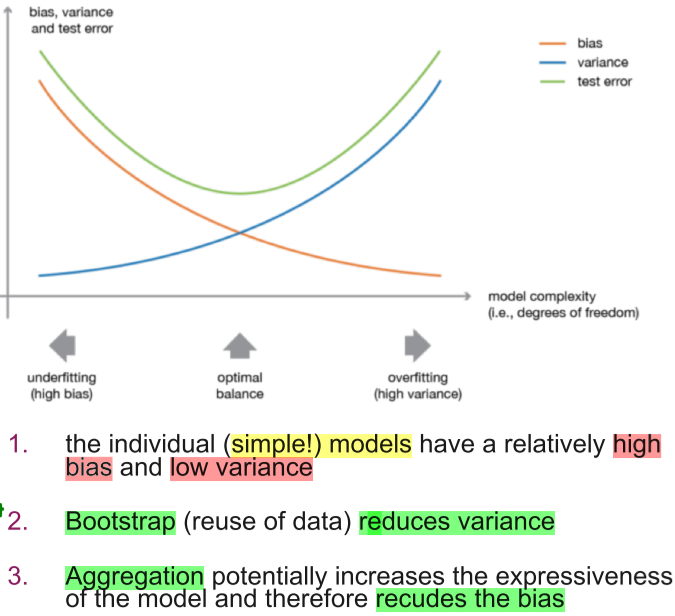
\includegraphics[width=0.75\linewidth]{./img/w13_bagging.png}

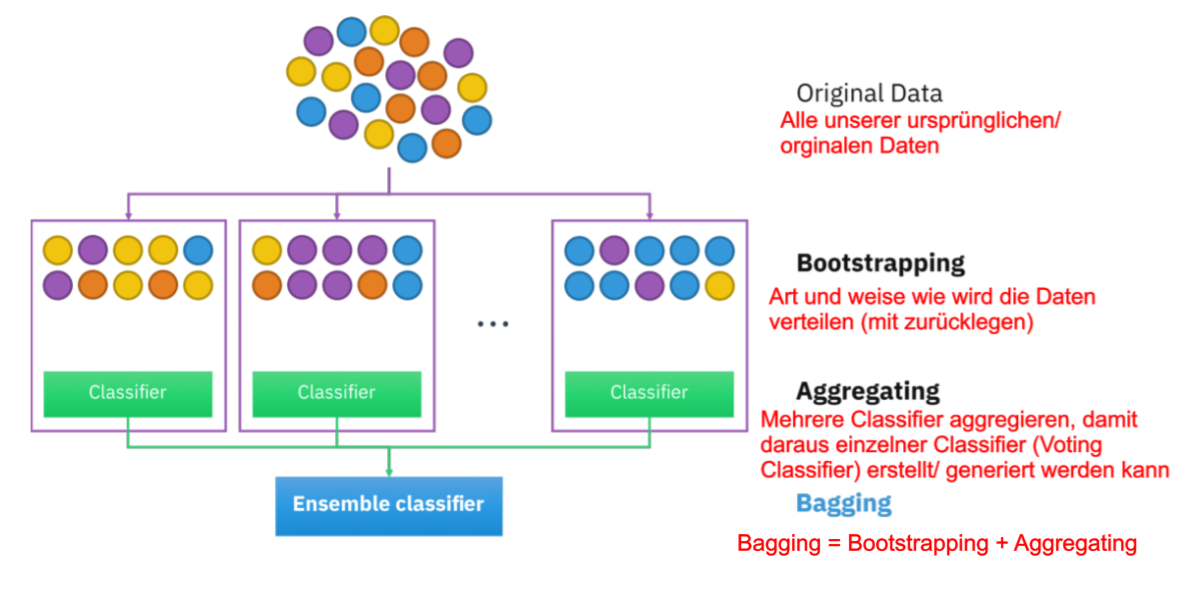
\includegraphics[width=\linewidth]{./img/bagging.png}

\subsubsection{Pasting}
In ML gibts nur Bagging, Pasting hat er nur als Gegenteil gebracht ist aber nicht relevant.
\begin{itemize}
    \item Wie Bagging nur: Sampling without replacement
\end{itemize}

\subsection{No free lunch theorem}
\textit{No single machine learning algorithm is universally the best-performing algorithm for all problems}
Some of the practical implications:
\begin{itemize}
    \item \textbf{No single algorithm} will solve all your machine learning problems better than every other algorithm
    \item Make sure you completely understand a machine learning problem and the data involved before selecting an algorithm to use
    \item All models are \textbf{only as good as the assumptions that they were created with} and the data that was used to train them
    \item \textbf{Simpler models like logistic regression have more bias and tend to \textit{underfit}, while more complex models like neural networks have more variance and tend to \textit{overfit}}
    \item The best models for a given problem are somewhere in the \textbf{middle of the two bias-variance extremes}
    \item To find a good model for a problem, you may have to \textbf{try different models and compare them using a robust cross-validation strategy}
\end{itemize}

\subsubsection{Training predictors (parallelization)}
\begin{itemize}
    \item If done sequentially can take too long. However, can be done in parallel!
    \item \python{ensemble_classifier = BaggingClassifier(..., n_jobs=-1) # -1=use all processors}
\end{itemize}

\subsubsection{Out of Bag (OOB) Evaluation}
Wenn Bagging verwendet wird, werden Werte eventuell mehrfach verwendet. Es kann aber auch Werte geben, welche gar nicht für das lernen verwendet wurden. Diese OOB-Daten sollen für die Überprüfung der Modelle angewendet werden.\\
\textbf{Vorteil:} Keine separate validation oder cross-validation nötig (aber es gibt am Schluss immer noch Test-Daten die gar nie verwendet wurden!)\\ 
\begin{minted}{python}
baggingRegressor = BaggingRegressor(base_estimator=LinearRegression(),
  n_estimators=50, 
  max_samples=0.05,  # each model is trained on 5% of the data (with replacement)
  max_features=6, # each model is sees only 6 (random) of 7 ftrs
  random_state=0, 
  oob_score = True # mit OOB
)
baggingRegressor = baggingRegressor.fit(X_train_scaled, y_train)

ensemble_classifier = BaggingClassifier(..., oob_score=True) # mit OOB
\end{minted}

\subsubsection{Different Features}
\begin{itemize}
    \item Different features can also be used for training predictors
    \item Bagging can be done on features as well
    \item Each predictor will be trained on  \textbf{random subesets} of the data features
    \item Sampling both features \& training data = \textbf{Random Patches}
    \item Sampling features only = \textbf{Random Subspaces}
\end{itemize}

\section{TI Befehle}
\begin{minipage}{0.5\linewidth}
\textbf{Skalarprodukt}
\begin{center}
    $Menu \rightarrow 7 \rightarrow C \rightarrow 3$\\
    $dotP\left(\begin{bmatrix}a \\ b\\ c\end{bmatrix}, \begin{bmatrix}d \\ e \\ f\end{bmatrix}\right)$
\end{center}
\end{minipage}
\begin{minipage}{0.49\linewidth}
\textbf{Normalisierungsvektor}
\begin{center}
    $Menu \rightarrow 7 \rightarrow 7 \rightarrow 1$\\
    $norm\left(\begin{bmatrix}a \\ b\\ c\end{bmatrix}\right)$
\end{center}
\end{minipage}

\begin{minipage}{0.5\linewidth}
\textbf{Ableiten/ Derivation}
\begin{center}
    $Menu \rightarrow 4 \rightarrow 1$\\
    $\frac{d}{dx}(5x)$
\end{center}
\end{minipage}
\begin{minipage}{0.49\linewidth}
\textbf{Integrieren}
\begin{center}
    $Menu \rightarrow 4 \rightarrow 3$\\
    $\int_{a}^{b} x^2,dx$
\end{center}
\end{minipage}

\textbf{Cosinus Distanz}
\begin{center}
    $cos(\theta) = \frac{dotP\left(\begin{bmatrix}a \\ b\\ c\end{bmatrix}, \begin{bmatrix}d \\ e \\ f\end{bmatrix}\right)}{norm\left(\begin{bmatrix}a \\ b\\ c\end{bmatrix}\right) * norm\left(\begin{bmatrix}d \\ e\\ f\end{bmatrix}\right)} \rightarrow Distanz (cos)$\\
    $\theta = cos^{-1}\left(\frac{dotP\left(\begin{bmatrix}a \\ b\\ c\end{bmatrix}, \begin{bmatrix}d \\ e \\ f\end{bmatrix}\right)}{norm\left(\begin{bmatrix}a \\ b\\ c\end{bmatrix}\right) * norm\left(\begin{bmatrix}d \\ e\\ f\end{bmatrix}\right)}\right) \rightarrow Distanz (Grad)$
\end{center}
